Thinking...
The user wants translation of Japanese sentence to English, but preserve TeX code as is. The Japanese text is:

"以下のの日本語文を英訳してください。ただしTeXのコードが挿入されているのでその部分はそのまま出力してください：" then the TeX block.

The TeX block contains a figure with caption: "新規出現高被引用テーマの高被引用テーマ全体に占める割合（\%）"

We need to translate the Japanese text outside TeX? Actually the request: "以下のの日本語文を英訳してください。ただしTeXのコードが挿入されているのでその部分はそのまま出力してください：" Then they provide the TeX code that includes Japanese caption. So we need to translate the Japanese caption to English while preserving the TeX code.

Thus output should be the same TeX block but with caption translated.

Original caption: "新規出現高被引用テーマの高被引用テーマ全体に占める割合（\%）"

Translation: "Proportion (%) of newly emerging highly cited themes among all highly cited themes". Could be "Percentage of newly emerging highly cited themes in the total of highly cited themes". Let's produce: "Percentage of newly emerging highly cited themes within the total highly cited themes (%)". The \% is inside parentheses.

Thus final output:

\begin{figure}[h]
\begin{center}
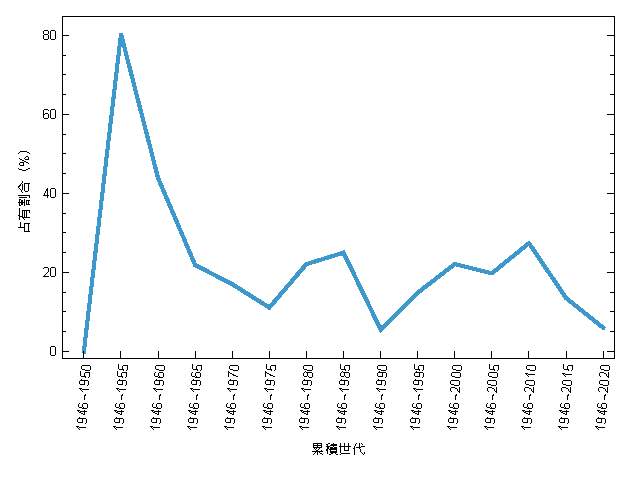
\includegraphics[width=76mm]{gr14.eps}
\caption{Percentage of newly emerging highly cited themes within the total highly cited themes (\%)} 
\label{fig:gr14}
\end{center}
\end{figure}

Make sure to keep formatting.

Also we might need to translate the surrounding Japanese instruction? Probably not; they ask to translate the Japanese sentence, which is the caption inside the TeX. So just output the translated TeX block.

Let's answer accordingly.
...done thinking.

\begin{figure}[h]
\begin{center}
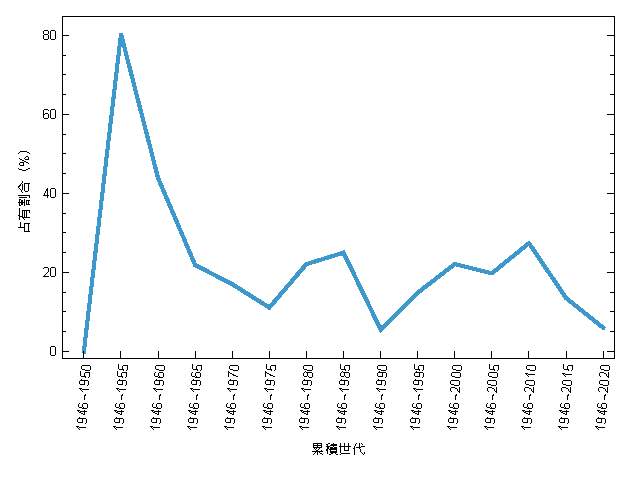
\includegraphics[width=76mm]{gr14.eps}
\caption{Percentage of newly emerging highly cited themes within the total highly cited themes (\%)} 
\label{fig:gr14}
\end{center}
\end{figure}

